\documentclass[fr]{../../../eplsummary}

\usepackage{../../../eplcommon}
\usepackage{../../../eplcode}
\lstset{language=Java}

\hypertitle[']{Algorithmique et structures de données}{5}{LSINF}{1121}
{Antoine Paris}
{Pierre Schauss}

\section{Piles, files et listes chaînées}
\subsection{Listes chaînées}
\paragraph{Définition} Une \textit{liste chaînée}
est une structure de données récursive qui est soit
vide (\textit{null}) soit une référence vers un
noeud contenant une donnée générique et une référence
vers une liste chaînée.

Pour définir un noeud, on utilise une classe imbriquée :

\begin{lstlisting}
private class Node {
	private Item item;
	private Node next;
}
\end{lstlisting}

Une liste chaînée permet, si on possède un lien vers
le premier et le dernier élément de réaliser les
opérations suivantes en un temps indépendant de la
taille de la liste :

\begin{itemize}
	\item Insérer un élément au début ;
	\item Supprimer un élément au début ;
	\item Insérer un élément à la fin.
\end{itemize}

Pour pouvoir effectuer des insertions/suppressions
arbitraires efficacement, il faut utiliser des listes
doublement chaînées (chaque noeud possède deux liens,
un dans chaque direction).

Les implémentations de \lstinline{Stack}, \lstinline{Queue}
et \lstinline{Bag} reposent sur les listes chaînées. Grâce
à ces dernières, l'espace mémoire requis est proportionnel
au nombre d'items dans la collection et le temps requis
par opération est toujours indépendant de la taille de la
collection (ce ne serait pas le cas en utilisant des tableaux
par exemple).

\subsection{Stack}
Le principe de fonctionnement d'une stack est illustré à la figure
\ref{fig:stack}.

\begin{figure}[ht]
	\centering
	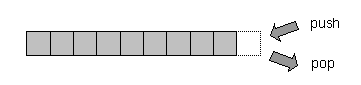
\includegraphics[scale=1.0]{img/stack.png}
	\caption{Illustration du fonctionnement d'une Stack LIFO.}
	\label{fig:stack}
\end{figure}

\lstinputlisting{code/Stack.java}

\subsection{Queue}
Le principe de fonctionnement d'une queue est illustré à la figure
\ref{fig:queue}.

\begin{figure}[ht]
	\centering
	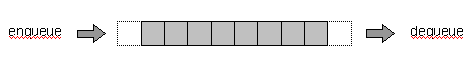
\includegraphics[scale=1.0]{img/queue.png}
	\caption{Illustration du fonctionnement d'une Queue FIFO.}
	\label{fig:queue}
\end{figure}

\lstinputlisting{code/Queue.java}

\subsection{Bag}
Un bag est simplement une stack sans méthode \lstinline{pop()}.

\section{Algorithmes de tri}
Le but du jeu ici est de trier des tableaux d'items contenant
chacun une clé en suivant un ordre bien particulier (le plus
souvent numérique ou alphabétique). La notion de clé est inclue
dans un mécanisme propre à Java, l'interface \lstinline{Comparable}
(et notamment la méthode \lstinline{compareTo}).

On distingue deux types d'algorithmes de tri, les algorithmes
\textbf{en place} qui n'utilisent pas (ou quasi pas) de mémoire
supplémentaire et ceux qui nécessitent assez de mémoire
supplémentaire pour garder une copie du tableau à trier en
mémoire.

Dans les algorthimes de tri présentés dans cette section,
on utilise le template suivant.

\lstinputlisting{code/SortTemplate.java}

\subsection{Selection Sort}
\subsubsection{Principe}
Le tri par sélection est un des plus simple. Il fonctionne
comme suit : premièrement, trouver l'élément le plus petit
du tableau et l'échanger avec le premier élément, ensuite
trouver le deuxième élément le plus petit du tableau et
l'échanger avec le deuxième élément, et ainsi de suite.
La traduction en Java est immédiate.

\subsubsection{Implémentation}
\lstinputlisting{code/Selection.java}

\subsubsection{Propriétés}
\paragraph{Le temps d'éxécution est indépendant de l'entrée}
L'algorithme mettra autant de temps à trier à tableau déjà
trié qu'un tableau aléatoirement ordonné.

\paragraph{Mouvement minimal}
Le nombre d'échange est une fonction linéaire de la taille
du tableau à trier ($N$ échanges sont effectués). 

\subsubsection{Complexité}
Dans tous les cas $\frac{N^2}{2}$ comparaisons et $N$ échanges.

\subsection{Insertion Sort}
\subsubsection{Principe}
C'est l'algorithme qu'on utilise en général pour trier
ses cartes. On considère une carte à la fois, et on
l'insère à sa place parmis les cartes déjà triées. La
seule différence est qu'ici il faut faire de la place
pour insérer l'item considéré à sa position, on doit
donc décaler tout les items plus grand que lui d'une
position vers la droite.

\subsubsection{Implémentation}
\lstinputlisting{code/Insertion.java}

\subsubsection{Propriétés}
Contrairement au tri par sélection, le temps d'éxécution
du tri par insertion est dépendant de l'entrée, il est par
exemple \textbf{excellent pour des tableaux presque triés}.

C'est également une méthode correcte pour de très petits
tableaux.

\subsubsection{Complexité}
Dans le pire cas, $\frac{N^2}{2}$ comparaisons et
$\frac{N^2}{2}$ échanges.

\subsection{Shell Sort}
\subsubsection{Principe}
Le shellsort est juste une simple extension du tri
par insertion. Dans le tri par insertion, les échanges
n'impliquent que des éléments adjacents, les items ne
peuvent donc se déplacer que d'un élément à la fois.
Le shellsort gagne en rapidité en autorisant des échanges
d'éléments éloignés dans le tableau.

\paragraph{Tableau $h$-trié} un tableau $h$-trié ($h$-sorted
array) est un tableau dont tous les éléments séparés
de $h$ positions sont triés.

\subsubsection{Implémentation}
Concrètement, l'algorithme s'implémente en utilisant le
tri par insertion pour obtenir successivement des 
tableaux $h$-triés avec $h$ décroissant.

\lstinputlisting{code/Shell.java}

\subsubsection{Propriétés}
Lorsqu'un tableau $h$-trié est $k$-trié, il reste
$h$-trié.

\subsubsection{Complexité}
Un peu moins quadratique, $N^{\frac{4}{3}}$, $N^{\frac{5}{4}}$
ou $N^{\frac{6}{5}}$ dans le pire cas.

\subsection{Mergesort}
Le principe du tri par fusion est assez simple : pour trier
un tableau, diviser le en deux moitiés, trier chaque moitié
(récursivement) et ensuite fusionner les résultats.

La complexité des algorithmes de tri par fusion est
logarithmique en $N\log N$. Le tri par fusion est
un algorithme de tri basé sur des comparaisons
asymptotiquement optimal (on ne peut pas faire mieux).

Les deux implémentations du tri par fusion vues ici
se base sur la méthode \lstinline{merge} suivante :

\lstinputlisting{code/mergeMethod.java}

\subsubsection{Top-down mergesort}
Ici, on divise le problème en sous-problèmes et on les résout
récursivement. 

\lstinputlisting{code/Merge.java}

\begin{figure}[ht]
	\centering
	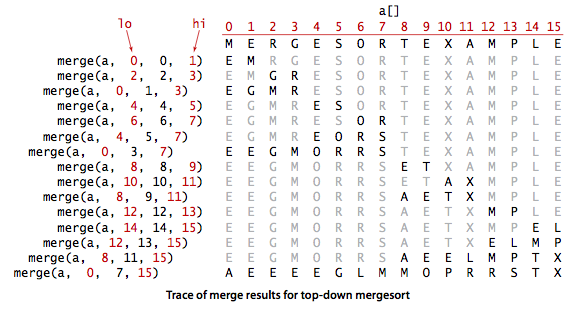
\includegraphics[scale=0.5]{img/mergesortTD.png}
	\caption{Trace des résultats de merge pour le top-down mergesort.}
\end{figure}

\subsubsection{Bottom-up mergesort}
Ici, on construit des petites solutions que l'on rassemble
pour en former des plus grandes à chaque fois. 

\lstinputlisting{code/MergeBU.java}

\begin{figure}[ht]
	\centering
	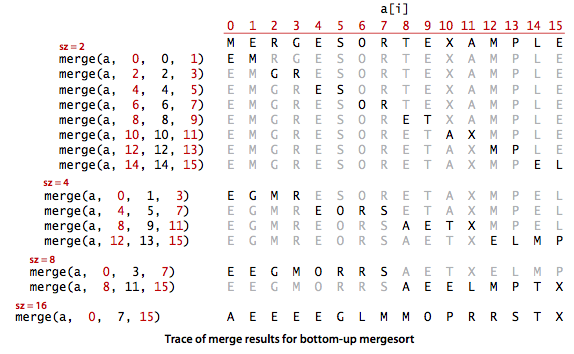
\includegraphics[scale=0.5]{img/mergesortBU.png}
	\caption{Trace des résultats de merge pour le bottom-up mergesort.}
\end{figure}

C'est la méthode à privilégier pour trier une liste chaînée.

\subsection{Quicksort}
Le tri rapide est probablement le plus utilisé, et ce pour
les deux raisons suivantes : il est en place et s'éxécute
en un temps proportionnel à $N \log N$.

\end{document}
